%!TEX root = da2020-07.tex

\Chapter{7}{Covering Maps}

\noindent
Chapters \chapterref{3}--\chapterref{6} have focused on positive results; now we will turn our attention to techniques that can be used to prove negative results. We will start with so-called covering maps\mydash we will use covering maps to prove that many problems cannot be solved at all with deterministic $\PN$-algorithms.

\section{Definition}

A covering map is a topological concept that finds applications in many areas of mathematics, including graph theory. We will focus on one special case: covering maps between port-numbered networks.

Let $N = (V,P,p)$ and $N' = (V'\!,P'\!,p')$ be port-numbered networks, and let $\phi \colon V \to V'$. We say that $\phi$ is a \emph{covering map from $N$ to $N'$} if the following holds:
\begin{enumerate}\raggedright
    \item $\phi$ is a surjection: $\phi(V) = V'$.
    \item $\phi$ preserves degrees: $\deg_{N}(v) = \deg_{N'}(\phi(v))$ for~all~$v \in V$.
    \item $\phi$ preserves connections and port numbers: $p(u,i) = (v,j)$ implies $p'(\phi(u),i) = (\phi(v),j)$.
\end{enumerate}
See Figures \ref{fig:covering-map}--\ref{fig:covering-map3} for examples.

\begin{figure}
    \centering
    \includegraphics[page=\PCoveringMap]{figs.pdf}
    \caption{There is a covering map $\phi$ from $N$ to $N'$ that maps $a_i \mapsto a$, $b_i \mapsto b$, $c_i \mapsto c$, and $d_i \mapsto d$ for each $i \in \{1, 2\}$.}\label{fig:covering-map}
\end{figure}

\begin{figure}
    \centering
    \includegraphics[page=\PCoveringMapB]{figs.pdf}
    \caption{There is a covering map $\phi$ from $N$ to $N'$ that maps $v_i \mapsto v$ for each $i \in \{1, 2, 3\}$. Here $N$ is a simple port-numbered network but $N'$ is not.}\label{fig:covering-map2}
\end{figure}

\begin{figure}
    \centering
    \includegraphics[page=\PCoveringMapC]{figs.pdf}
    \caption{There is a covering map $\phi$ from $N$ to $N'$ that maps $v_i \mapsto v$ for each $i \in \{1, 2\}$. Again, $N$ is a simple port-numbered network but $N'$ is not.}\label{fig:covering-map3}
\end{figure}

We can also consider labeled networks, for example, networks with local inputs. Let $f\colon V \to X$ and $f'\colon V' \to X$. We say that $\phi$ is a covering map from $(N,f)$ to $(N'\!,f')$ if $\phi$ is a covering map from $N$ to $N'$ and the following holds:
\begin{enumerate}[resume*]
    \item $\phi$ preserves labels: $f(v) = f'(\phi(v))$ for all $v \in V$.
\end{enumerate}

\section{Covers and Executions}

Now we will study covering maps from the perspective of deterministic $\PN$-algorithms. The basic idea is that a covering map $\phi$ from $N$ to $N'$ fools any $\PN$-algorithm $A$: a node $v$ in $N$ is indistinguishable from the node $\phi(v)$ in $N'$.

Without further ado, we state the main result and prove it\mydash many applications and examples will follow.

\begin{theorem}\label{thm:cover}
    Assume that
    \begin{enumerate}[itemsep=0ex]\raggedright
        \item $A$ is a deterministic $\PN$-algorithm with $X = \Input_A$,
        \item $N = (V,P,p)$ and $N' = (V'\!,P'\!,p')$ are port-numbered networks,
        \item $f\colon V \to X$ and $f'\colon V' \to X$ are arbitrary functions, and
        \item $\phi\colon V \to V'$ is a covering map from $(N,f)$ to $(N'\!,f')$.
    \end{enumerate}
    Let
    \begin{enumerate}[resume*]
        \item $x_0, x_1, \dotsc$ be the execution of $A$ on $(N,f)$, and
        \item $x'_0, x'_1, \dotsc$ be the execution of $A$ on $(N'\!,f')$.
    \end{enumerate}
    Then for each $t = 0, 1, \dotsc$ and each $v \in V$ we have $x_t(v) = x'_t(\phi(v))$.
\end{theorem}

\begin{proof}
    We will use the notation of Section~\longref{3.3.2}{ssec:execution}; the symbols with a prime refer to the execution of $A$ on $(N'\!,f')$. In particular, $m'_t(u',i)$ is the message received by $u' \in V'$ from port $i$ in round $t$ in the execution of $A$ on $(N'\!,f')$, and $m'_t(u')$ is the vector of messages received by $u'$.
    
    The proof is by induction on $t$. To prove the base case $t = 0$, let $v \in V$, $d = \deg_N(v)$, and $v' = \phi(v)$; we have
    \[
        x'_0(v') = \Init_{A,d}(f'(v')) = \Init_{A,d}(f(v)) = x_0(v).
    \]
    
    For the inductive step, let $(u,i) \in P$, $(v,j) = p(u,i)$, $d = \deg_N(u)$, $\ell = \deg_N(v)$, $u' = \phi(u)$, and $v' = \phi(v)$. Let us first consider the messages sent by $v$ and $v'$; by the inductive assumption, these are equal:
    \[
        \Send_{A,\ell}(x'_{t-1}(v')) = \Send_{A,\ell}(x_{t-1}(v)).
    \]
    
    A covering map $\phi$ preserves connections and port numbers: $(u,i) = p(v,j)$ implies $(u',i) = p'(v',j)$. Hence $m_t(u,i)$ is component $j$ of $\Send_{A,\ell}(x_{t-1}(v))$, and $m'_t(u',i)$ is component $j$ of $\Send_{A,\ell}(x'_{t-1}(v'))$. It follows that $m_t(u,i) = m'_t(u',i)$ and $m_t(u) = m'_t(u')$. Therefore
    \begin{align*}
        x'_t(u')
        &= \Receive_{A,d}\bigl(x'_{t-1}(u'), m'_t(u') \bigr) \\
        &= \Receive_{A,d}\bigl(x_{t-1}(u), m_t(u) \bigr)
        = x_t(u). \qedhere
    \end{align*}
\end{proof}

In particular, if the execution of $A$ on $(N,f)$ stops in time $T$, the execution of $A$ on $(N'\!,f')$ stops in time $T$ as well, and vice versa. Moreover, $\phi$ preserves the local outputs: $x_T(v) = x'_T(\phi(v))$ for all $v \in V$.

\section{Examples}

We will give representative examples of negative results that we can easily derive from Theorem~\ref{thm:cover}. First, we will observe that a deterministic $\PN$-algorithm cannot break symmetry in a cycle\mydash unless we provide some symmetry-breaking information in local inputs.

\begin{lemma}\label{lem:cycle-symmetric}
    Let $G = (V,E)$ be a cycle graph, let $A$ be a deterministic $\PN$-algorithm, and let $f$ be a constant function $f\colon V \to \{0\}$. Then there is a simple port-numbered network $N = (V,P,p)$ such that
    \begin{enumerate}
        \item the underlying graph of $N$ is $G$, and
        \item if $A$ stops on $(N,f)$, the output is a constant function $g\colon V \to \{c\}$ for some $c$.
    \end{enumerate}
\end{lemma}
\begin{proof}
    Label the nodes $V = \Set{ v_1, v_2, \dotsc, v_n }$ along the cycle so that the edges are
    \[
        E = \bigSet{ \{v_1, v_2\},\ \{v_2, v_3\},\ \dotsc,\ \{v_{n-1}, v_n\},\ \{v_n, v_1\} }.
    \]
    Choose the port numbering $p$ as follows:
    \begin{align*}
        p\colon &(v_1, 1) \mapsto (v_2, 2),\ (v_2, 1) \mapsto (v_3, 2),\ \dotsc, \\
                &(v_{n-1}, 1) \mapsto (v_n, 2),\ (v_n, 1) \mapsto (v_1, 2).
    \end{align*}
    See Figure~\ref{fig:covering-map2} for an illustration in the case $n = 3$.
    
    Define another port-numbered network $N' = (V'\!,P'\!,p')$ with $V' = \{v\}$, $P' = \{ (v,1), (v,2) \}$, and $p(v,1) = (v,2)$. Let $f'\colon V' \to \{0\}$. Define a function $\phi\colon V \to V'$ by setting $\phi(v_i) = v$ for each $i$.
    
    Now we can verify that $\phi$ is a covering map from $(N,f)$ to $(N'\!,f')$. Assume that $A$ stops on $(N,f)$ and produces an output~$g$. By Theorem~\ref{thm:cover}, $A$ also stops on $(N'\!,f')$ and produces an output~$g'$. Let $c = g'(v)$. Now
    \[
        g(v_i) = g'(\phi(v_i)) = g'(v) = c
    \]
    for all~$i$.
\end{proof}

In the above proof, we never assumed that the execution of $A$ on $N'$ makes any sense\mydash after all, $N'$ is not even a simple port-numbered network, and there is no underlying graph. Algorithm $A$ was never designed to be applied to such a strange network with only one node. Nevertheless, the execution of $A$ on $N'$ is formally well-defined, and Theorem~\ref{thm:cover} holds. We do not really care what $A$ outputs on $N'$, but the existence of a covering map can be used to prove that the output of $A$ on $N$ has certain properties. It may be best to interpret the execution of $A$ on $N'$ as a thought experiment, not as something that we would actually try to do in practice.

Lemma~\ref{lem:cycle-symmetric} has many immediate corollaries.

\begin{corollary}\label{cor:cycle-symmetric}
    Let $\calF$ be the family of cycle graphs. Then there is no deterministic $\PN$-algorithm that solves any of the following problems on~$\calF$:
    \begin{enumerate}[noitemsep]
        \item maximal independent set,
        \item \Apx{1.999} of a minimum vertex cover,
        \item \Apx{2.999} of a minimum dominating set,
        \item maximal matching,
        \item vertex coloring,
        \item weak coloring,
        \item edge coloring.
    \end{enumerate}
\end{corollary}
\begin{proof}
    In each of these cases, there is a graph $G \in \calF$ such that a constant function is not a feasible solution in the network $N$ that we constructed in Lemma~\ref{lem:cycle-symmetric}.
    
    For example, consider the case of dominating sets; other cases are similar. Assume that $G = (V,E)$ is a cycle with $3k$ nodes. Then a minimum dominating set consists of $k$ nodes\mydash it is sufficient to take every third node. Hence a \Apx{2.999} of a minimum dominating set consists of at most $2.999k < 3k$ nodes. A solution $D = V$ violates the approximation guarantee, as $D$ has too many nodes, while $D = \emptyset$ is not a dominating set. Hence if $A$ outputs a constant function, it cannot produce a \Apx{2.999} of a minimum dominating set.
\end{proof}

\begin{lemma}
    There is no deterministic $\PN$-algorithm that finds a weak coloring for every \Reg{3} graph.
\end{lemma}
\begin{proof}
    Again, we are going to apply the standard technique: pick a suitable \Reg{3} graph $G$, find a port-numbered network $N$ that has $G$ as its underlying graph, find a smaller network $N'$ such that we have a covering map $\phi$ from $N$ to $N'$, and apply Theorem~\ref{thm:cover}.
    
    However, it is not immediately obvious which \Reg{3} graph would be appropriate; hence we try the simplest possible case first. Let $G = (V,E)$ be the \emph{complete graph} on four nodes: $V = \Set{s,t,u,v}$, and we have an edge between any pair of nodes; see Figure~\ref{fig:three-reg}. The graph is certainly \Reg{3}: each node is adjacent to the other three nodes.

    \begin{figure}
        \centering
        \includegraphics[page=\PThreeReg]{figs.pdf}
        \caption{Graph $G$ is the complete graph on four nodes. The edges of $G$ can be partitioned into a $2$-factor $X$ and a $1$-factor $Y$. Network $N$ has $G$ as its underlying graph, and there is a covering map $\phi$ from $N$ to $N'$}\label{fig:three-reg}
    \end{figure}
        
    Now it is easy to verify that the edges of $G$ can be partitioned into a $2$-factor $X$ and a $1$-factor $Y$. The $2$-factor consists of a cycle and a $1$-factor consists of disjoint edges. We can use the factors to guide the selection of port numbers in~$N$.
    
    In the cycle induced by $X$, we can choose symmetric port numbers using the same idea as what we had in the proof of Lemma~\ref{lem:cycle-symmetric}; one end of each edge is connected to port $1$ while the other end is connected to port $2$. For the edges of the $1$-factor $Y$, we can assign port number $3$ at each end. We have constructed the port-numbered network $N$ that is illustrated in Figure~\ref{fig:three-reg}.
    
    Now we can verify that there is a covering map $\phi$ from $N$ to $N'$, where $N'$ is the network with one node illustrated in Figure~\ref{fig:three-reg}. Therefore in any algorithm $A$, if we do not have any local inputs, all nodes of $N$ will produce the same output. However, a constant output is not a weak coloring of $G$.
\end{proof}

In the above proof, we could have also partitioned the edges of $G$ into three $1$-factors, and we could have used the $1$-factorization to guide the selection of port numbers. However, the above technique is more general: there are \Reg{3} graphs that do not admit a $1$-factorization but that can be partitioned into a $1$-factor and a $2$-factor.

So far we have used only one covering map in our proofs; the following lemma gives an example of the use of more than one covering map.

\begin{lemma}\label{lem:cycles-and-covers}
    Let $\calF = \Set{G_3, G_4}$, where $G_3$ is the cycle graph with $3$ nodes, and $G_4$ is the cycle graph with $4$ nodes. There is no deterministic $\PN$-algorithm that solves the following problem $\Pi$ on $\calF$: in $\Pi(G_3)$ all nodes output $3$ and in $\Pi(G_4)$ all nodes output $4$.
\end{lemma}
\begin{proof}
    We again apply the construction of Lemma~\ref{lem:cycle-symmetric}; for each $i \in \{3,4\}$, let $N_i$ be the symmetric port-numbered network that has $G_i$ as the underlying graph.
    
    Now it would be convenient if we could construct a covering map from $N_4$ to $N_3$; however, this is not possible (see the exercises). Therefore we proceed as follows. Construct a one-node network $N'$ as in the proof of Lemma~\ref{lem:cycle-symmetric}, construct the covering map $\phi_3$ from $N_3$ to $N'$, and construct the covering map $\phi_4$ from $N_4$ to $N'$; see Figure~\ref{fig:cycles-and-covers}. The local inputs are assumed to be all zeros.

    \begin{figure}
        \centering
        \includegraphics[page=\PCyclesAndCovers]{figs.pdf}
        \caption{The structure of the proof of Lemma~\ref{lem:cycles-and-covers}.}\label{fig:cycles-and-covers}
    \end{figure}
    
    Let $A$ be a $\PN$-algorithm, and let $c$ be the output of the only node of $N'$. If we apply Theorem~\ref{thm:cover} to $\phi_3$, we conclude that all nodes of $N_3$ output $c$; if $A$ solves $\Pi$ on $G_3$, we must have $c = 3$. However, if we apply Theorem~\ref{thm:cover} to $\phi_4$, we learn that all nodes of $N_4$ also output $c = 3$, and hence $A$ cannot solve $\Pi$ on $\calF$.
\end{proof}

We have learned that a deterministic $\PN$-algorithm cannot determine the length of a cycle. In particular, a deterministic $\PN$-algorithm cannot determine if the underlying graph is bipartite.


\section{Quiz}

Let $G = (V, E)$ be a graph. A set $X \subseteq V$ is a \emph{$k$-tuple dominating set} if for every $v \in V$ we have $|\ball_G(v,1) \cap X| \ge k$. Consider the problem of finding a minimum 2-tuple dominating set in \emph{cycles}. What is the best (i.e.\ smallest) approximation ratio we can achieve in the $\PN$ model?


\section{Exercises}

We use the following definition in the exercises. A graph $G$ is \emph{homogeneous} if there are port-numbered networks $N$ and $N'$ and a covering map $\phi$ from $N$ to $N'$ such that $N$ is simple, the underlying graph of $N$ is $G$, and $N'$ has only one node. For example, Lemma~\ref{lem:cycle-symmetric} shows that all cycle graphs are homogeneous.

\begin{ex}[finding port numbers]\label{ex:cover-three-reg1}
    Consider the graph $G$ and network $N'$ illustrated in Figure~\ref{fig:cover-ex-three-reg}. Find a simple port-numbered network $N$ such that $N$ has $G$ as the underlying graph and there is a covering map from $N$ to $N'$.

    \begin{figure}
        \centering
        \includegraphics[page=\PCoverExThreeReg]{figs.pdf}
        \caption{Graph $G$ and network $N'$ for Exercises \ref{ex:cover-three-reg1} and \ref{ex:cover-reg}b.}\label{fig:cover-ex-three-reg}
    \end{figure}
\end{ex}

\begin{ex}[homogeneity]
    Assume that $G$ is homogeneous and it contains a node of degree at least two. Give several examples of graph problems that cannot be solved with any deterministic $\PN$-algorithm in any family of graphs that contains $G$.
\end{ex}

\begin{ex}[regular and homogeneous]\label{ex:cover-reg}
    Show that the following graphs are homogeneous:
    \begin{subex}
        \item graph $G$ illustrated in Figure~\ref{fig:cover-ex-four-reg},
        \item graph $G$ illustrated in Figure~\ref{fig:cover-ex-three-reg}.
    \end{subex}

    \hint{(a)~Apply the result of Exercise~\longref{2.8}{ex:2fact}. (b)~Find a $1$-factor.}

    \begin{figure}
        \centering
        \includegraphics[page=\PCoverExFourReg]{figs.pdf}
        \caption{Graph $G$ for Exercise~\ref{ex:cover-reg}a.}\label{fig:cover-ex-four-reg}
    \end{figure}
\end{ex}

\begin{ex}[complete graphs]\label{ex:cover-complete}
    Recall that we say that a graph $G = (V,E)$ is \emph{complete} if for all nodes $u, v \in V$, $u \ne v$, there is an edge $\{u,v\} \in E$. Show that
    \begin{subex}
        \item any $2k$-regular graph is homogeneous,
        \item any complete graph with $2k$ nodes has a $1$-factorization,
        \item any complete graph is homogeneous.
    \end{subex}
\end{ex}

\begin{ex}[dominating sets]\label{ex:domset}
    Let $\Delta \in \{2,3,\dotsc\}$, let $\epsilon > 0$, and let $\calF$ consist of all graphs of maximum degree at most $\Delta$. Show that it is possible to find a \Apx{(\Delta+1)} of a minimum dominating set in constant time in family~$\calF$ with a deterministic $\PN$-algorithm. Show that it is not possible to find a \Apx{(\Delta+1-\epsilon)} with a deterministic $\PN$-algorithm.
    
    \hint{For the lower bound, use the result of Exercise~\ref{ex:cover-complete}c.}
\end{ex}

\begin{ex}[covers with covers]\label{ex:cover-cover}
    What is the connection between covering maps and the vertex cover 3-approximation algorithm in Section~\longref{3.6}{sec:vc3}?
\end{ex}

\begin{exs}[\Reg{3} and not homogeneous]\label{ex:cover-three-reg-b}
    Consider the graph $G$ illustrated in Figure~\ref{fig:cover-ex-three-reg-b}.
    \begin{subex}
        \item Show that $G$ is not homogeneous.
        \item Present a deterministic $\PN$-algorithm $A$ with the following property: if $N$ is a simple port-numbered network that has $G$ as the underlying graph, and we execute $A$ on $N$, then $A$ stops and produces an output where at least one node outputs $0$ and at least one node outputs $1$.
        \item Find a simple port-numbered network $N$ that has $G$ as the underlying graph, a port-numbered network $N'$, and a covering map $\phi$ from $N$ to $N'$ such that $N'$ has the smallest possible number of nodes.
    \end{subex}
    \hint{Show that if a \Reg{3} graph is homogeneous, then it has a $1$-factor. Show that $G$ does not have any $1$-factor.}

    \begin{figure}
        \centering
        \includegraphics[page=\PCoverExThreeRegB]{figs.pdf}
        \caption{Graph $G$ for Exercise~\ref{ex:cover-three-reg-b}.}\label{fig:cover-ex-three-reg-b}
    \end{figure}
\end{exs}

\begin{exs}[covers and connectivity]
    Assume that $N = (V,P,p)$ and $N' = (V'\!,P'\!,p')$ are simple port-numbered networks such that there is a covering map $\phi$ from $N$ to $N'$. Let $G$ be the underlying graph of network $N$, and let $G'$ be the underlying graph of network~$N'$.
    \begin{subex}
        \item Is it possible that $G$ is connected and $G'$ is not connected?
        \item Is it possible that $G$ is not connected and $G'$ is connected?
    \end{subex}
\end{exs}

\begin{exs}[$k$-fold covers]
    Let $N = (V,P,p)$ and $N' = (V'\!,P'\!,p')$ be simple port-numbered networks
    such that the underlying graphs of $N$ and $N'$ are connected, and
    assume that $\phi\colon V \to V'$ is a covering map from $N$ to $N'$.
    Prove that there exists a positive integer $k$ such that the following holds:
    $|V| = k |V'|$ and for each node $v' \in V'$ we have $|\phi^{-1}(v')| = k$.
    Show that the claim does not necessarily hold if the underlying graphs are not connected.
\end{exs}


\section{Bibliographic Notes}

The use of covering maps in the context of distributed algorithm was introduced by Angluin~\cite{angluin80local}. The general idea of Exercise~\ref{ex:cover-three-reg-b} can be traced back to Yamashita and Kameda~\cite{yamashita96computing}, while the specific construction in Figure~\ref{fig:cover-ex-three-reg-b} is from Bondy and Murty's textbook~\cite[Figure~5.10]{bondy76graph-theory}. Parts of exercises \ref{ex:cover-three-reg1}, \ref{ex:cover-reg}, \ref{ex:cover-complete}, and \ref{ex:domset} are inspired by our work \cite{suomela10eds,astrand10weakly-coloured}.
